%!TEX program = lualatex

\documentclass[10pt]{article}
\usepackage[margin=1in]{geometry}
\usepackage{fontawesome}
\usepackage{fontspec}
\usepackage[hidelinks]{hyperref}
\usepackage{pdfpages}
\usepackage{csquotes}
\usepackage{ragged2e}
\MakeOuterQuote{"}
\setmainfont[Numbers=OldStyle]{Crimson Text}
\setsansfont{Gill Sans MT}
\setmonofont{Deja Vu Sans Mono}
\usepackage{microtype}
\usepackage{color}
\usepackage{lettrine}
\usepackage{booktabs}
\usepackage{array,multirow}

\setlength{\parindent}{0em}
\setlength{\parskip}{10pt}

\definecolor{fsuMaroon}{RGB}{155,0,33}

\newcommand{\dueDate}[1]{\textbf{\textcolor{fsuMaroon}{#1}}}
\newcommand{\subHead}[1]{\noindent\textbf{\textsf{\textcolor{fsuMaroon}{#1}}}}
\newcommand{\dueCalendar}{\noindent\lettrine{\dueDate{\faCalendar}}{~~}}
\newcommand{\dueText}[1]{\normalsize\textsf{#1}}
\newcommand{\bottomRule}{\vfill\begin{center}\rule{4in}{1pt}\end{center}}

\begin{document}

\begin{center}
\noindent\Large\dueDate{\faBriefcase}~~\textsf{\textit{EDUC1199 Project Package:} 48-Hour Social-Emotional Journal}~~\dueDate{\faBook}\normalsize\\
\rule{5.5in}{1pt}
\end{center}

As a way to engage in constructing digital learning environments and “getting your feet wet” using the Teaching for Understanding framework, you will construct a well-structured WebQuest for elementary (3rd grade or above), middle, high school, or adult pupils on a particular topic of your choosing. We will be using the Zunal WebQuest Builder.

\subHead{Your WebQuest Should Include:}
\begin{itemize}
	\itemsep-0.5em
	\item The following pages of a WebQuest: Welcome, Introduction, Task, Process, Evaluation and Conclusion.
	\item An image on every page of the WebQuest (such as those from \url{http://bit.ly/2201-images} or \url{http://photosforclass.com/}).
	\item A good generative topic and 2-3 understanding goals to guide your WebQuest in the Introduction.
	\item A Task page that provides an overview of the "big project" (culminating performance).
	\item A Process with roles, at least one introductory performance, at least one intermediate performances, and one culminating performance.
	\item An Evaluation that lists 2-3 criteria that you would be looking at to evaluate students' understandings.
	\item A Conclusion that includes an opportunity for students to reflect on their learning and understanding, including questions to help students think about their learning in new situations.

\end{itemize}

\subHead{Your WebQuest Reflection Write-Up Should Include:}
Here's what you need in your reflection paper, which should be 1-2 pages long, single-spaced:

\begin{itemize}
	\itemsep-0.5em
	\item A description of how the generative topic and the understanding goals guided your WebQuest.
	\item Imagine and report (see Course Tools and Practices document) how a teacher might use your WebQuest: how might it be introduced? How might the teacher encourage her students to use it?
	\item \textbf{IF YOU ARE WORKING AS A PAIR:} A description of what you contributed to your WebQuest team, and a plan for how you might do things better in your group in the future.
\end{itemize}

\subHead{Remember The Framework}

This is a list of projects from prior semesters that represent a range of disciplines and grade levels. Although I consider all of these to be very good examples, make sure you evaluate these models yourself and determine what you can learn from these models.

\footnotesize\centering\begin{tabular}{p{2in}p{2in}p{2in}}
	\toprule
	\multirow{9}{*}{\parbox[l]{5cm}{\raggedright\Large New Haven Social Development Curriculum \footnotesize}} & \multirow{3}{*}{\normalsize Skills \footnotesize} & Self-Management \\
	 & & Problem Solving and Decision Making \\
	 & & Communication \\
	\cline{2-3}
	 & \multirow{3}{*}{\normalsize Attitudes and Values \footnotesize} & About Self \\
	 & & About Others \\
	 & & About Tasks \\
	 \cline{2-3}
	 & \multirow{3}{*}{\normalsize Content \footnotesize} & Self/Health \\
	 & & Relationships \\
	 & & School/Community \\
	 \bottomrule
\end{tabular}\justifying

\vfill

\dueCalendar\dueText{\dueDate{Your 48-Hour Social-Emotional Journal are due in TaskStream by August 31.} No late work will be accepted without prior approval. Please let me know if you have any questions whatsoever. I look forward to reading your insights!}
\newpage

\centering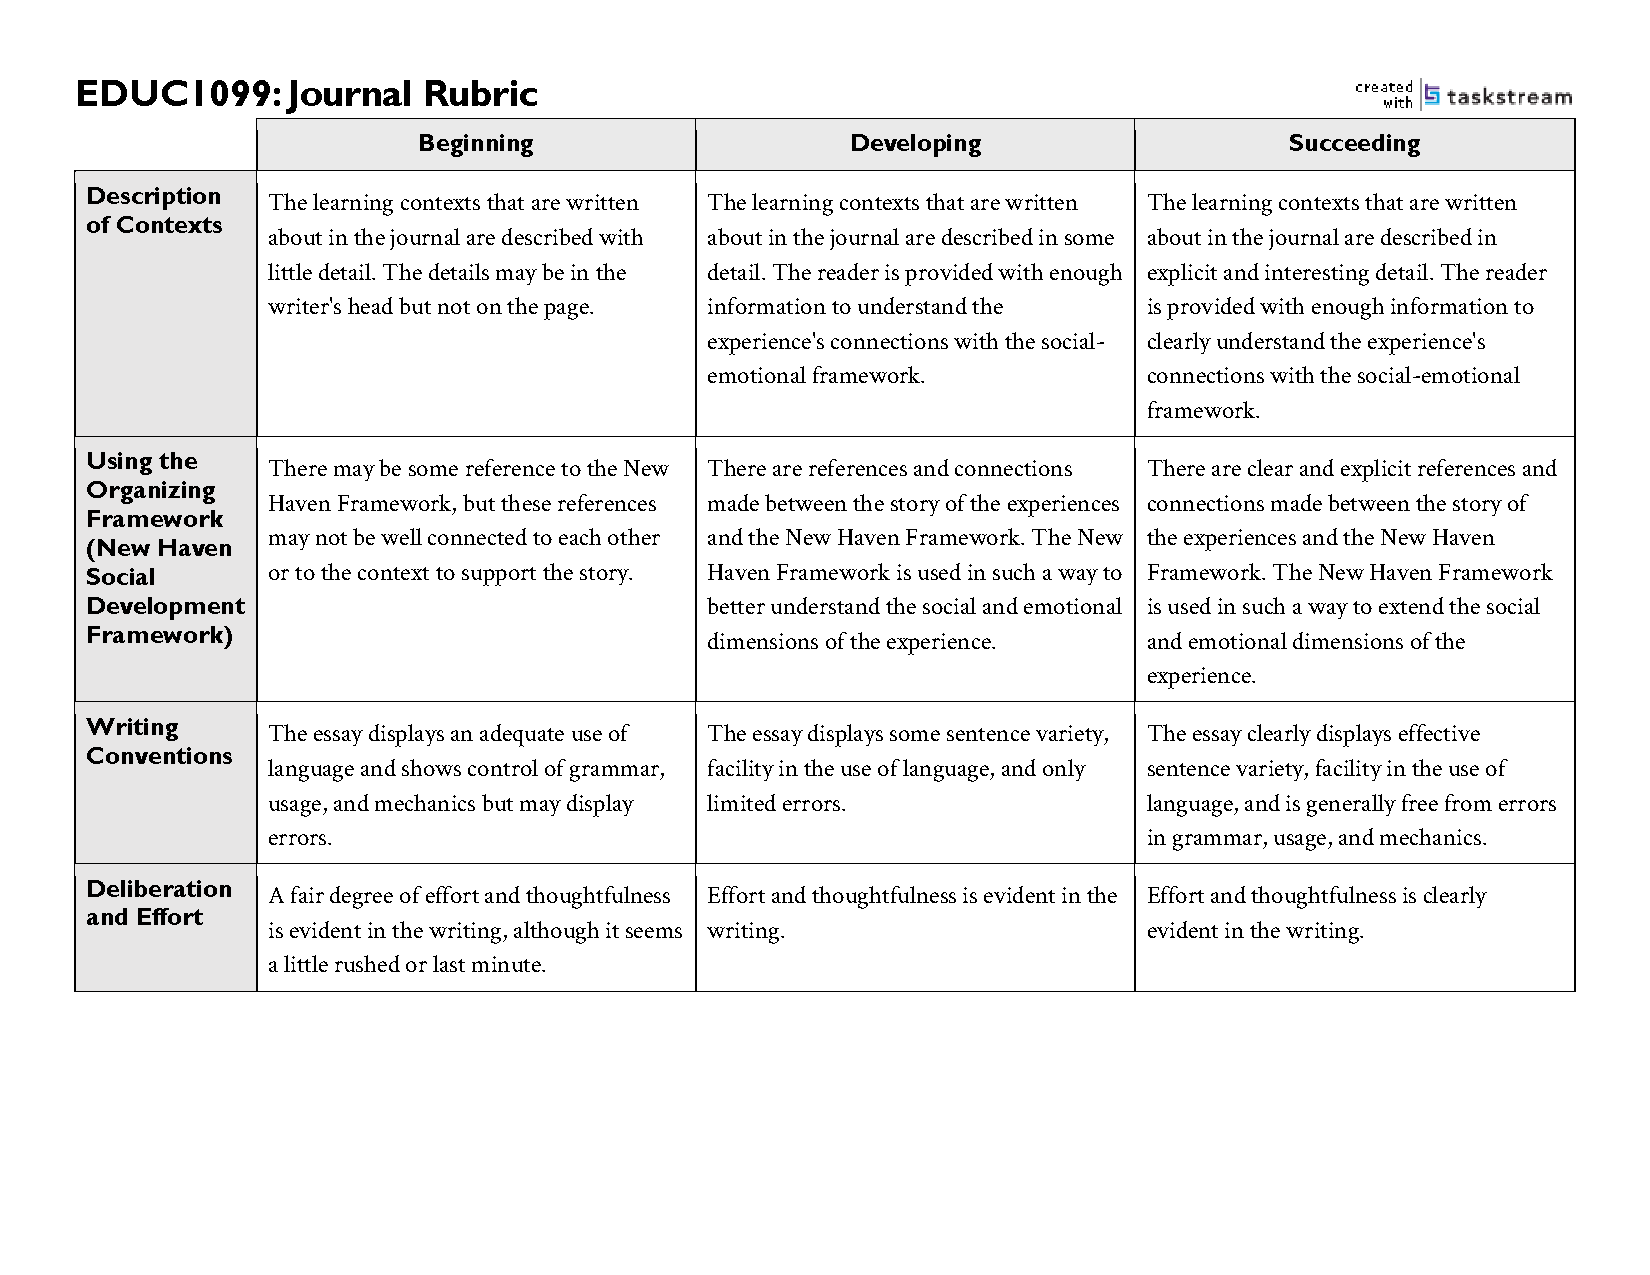
\includepdf[angle=90,width=8in]{journal-rubric.pdf}

\end{document}
